\chapter{Compositions of Functions}

Given $f(x) = x^2 + 5$ and $g(x) = -3x-2$, find or evaluate each.

\begin{multicols}{4}
\begin{enumerate}
	\item $(f \circ g)(x)$
	\item $(g \circ f)(x)$
	\item $(f \circ f)(x)$
	\item $g(g(x))$
\end{enumerate}	\setcounter{Review}{\value{enumi}}
\end{multicols}
\begin{multicols}{4}
\begin{enumerate}		\setcounter{enumi}{\value{Review}}
	\item $(f \circ g)(1)$
	\item $(g \circ f)(-2)$
	\item $(f \circ f)(0)$
	\item $g(g(-8))$
\end{enumerate}	\setcounter{Review}{\value{enumi}}
\end{multicols}

Given the graph of $f(x)$ and $g(x)$, find each.
\begin{center}
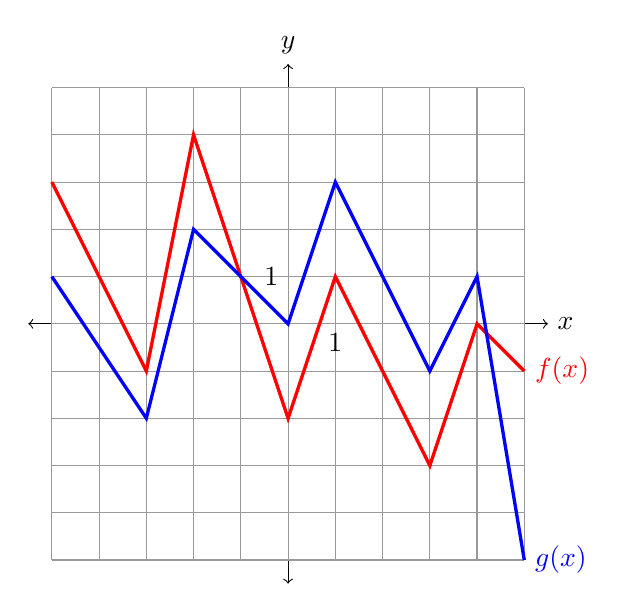
\begin{tikzpicture}[scale=0.6]
\draw[<->] (-5.5,0) -- (5.5,0) node [right] {$x$};
\draw[<->] (0,-5.5) -- (0,5.5) node [above] {$y$};
\draw[gray!80] (-5,-5) grid (5,5);
\node at (1,0) [below] {$1$};
\node at (0,1) [left] {$1$};
\coordinate (A) at (-5,3);
\coordinate (B) at (-3,-1);
\coordinate (C) at (-2,4);
\coordinate (D) at (0,-2);
\coordinate (E) at (1,1);
\coordinate (F) at (3,-3);
\coordinate (G) at (4,0);
\coordinate (H) at (5,-1);
\draw[red, very thick] (A) -- (B) -- (C) -- (D) -- (E) -- (F) -- (G) -- (H) node [right] {$f(x)$};
\coordinate (I) at (-5,1);
\coordinate (J) at (-3,-2);
\coordinate (K) at (-2,2);
\coordinate (L) at (0,0);
\coordinate (M) at (1,3);
\coordinate (N) at (3,-1);
\coordinate (O) at (4,1);
\coordinate (P) at (5,-5);
\draw[blue, very thick] (I) -- (J) -- (K) -- (L) -- (M) -- (N) -- (O) -- (P) node [right] {$g(x)$};
\end{tikzpicture}
\end{center}

\begin{multicols}{4}
\begin{enumerate}	\setcounter{enumi}{\value{Review}}
	\item $(f \circ g)(0)$
	\item $(g \circ f)(-5)$
	\item $(f \circ f)(1)$
	\item $(g(g(5))$
\end{enumerate}	\setcounter{Review}{\value{enumi}}
\end{multicols}

\newpage

\section*{Answer Key}

\begin{enumerate}
	\item $9x^2+12x+9$
    \item $-3x^2-17$
    \item $x^4+10x^2+30$
    \item $9x+4$
    \item 30
    \item $-29$
    \item 30
    \item $-68$
    \item $-2$
    \item $-1$
    \item 1
    \item 1
\end{enumerate}